\documentclass{ifto-tex}

\usepackage{gensymb}
\usepackage{lmodern}			% Usa a fonte Latin Modern
\usepackage[T1]{fontenc}		% Selecao de codigos de fonte.
\usepackage[utf8]{inputenc}		% Codificacao do documento (conversão automática dos acentos)
\usepackage{indentfirst}		% Indenta o primeiro parágrafo de cada seção.
\usepackage{color}				% Controle das cores
\usepackage{graphicx}			% Inclusão de gráficos
\usepackage{microtype} 			% para melhorias de justificação
\usepackage{float}
\usepackage{longtable}

% Uso da fonte Arial (IFTO)
\usepackage{helvet}
\renewcommand{\familydefault}{\sfdefault}

\usepackage[brazilian,hyperpageref]{backref}	 % Paginas com as citações na bibl
\usepackage[alf,
versalete,
abnt-emphasize = bf, % destaca o titulo em negrito;
abnt-etal-list = 3, % trabalhos com mais de 3 autores recebem et al.,;
abnt-etal-text = it, % escreve o et al., em italico;
abnt-and-type = &, % usa o carater '&' no lugar de 'e' para mais de um autor;
abnt-last-names = abnt, % trata sobrenomes 'estritamente' conforme a ABNT; e
abnt-repeated-author-omit = yes % autores com + de uma entrada recebem '____.'
]{abntex2cite}

% Configuração das referências bibliográficas
\renewcommand{\backref}{}
\renewcommand*{\backrefalt}[4]{	}


%%%%%%%%%%%%%%%%%%%%%%%%%%%%%%%%%%%%%%%%%%%%%%%%%%%%%%%%%%%%%%%%%%%%%%%%%%%%%%%%
% Informações da capa e da folha de rosto
%%%%%%%%%%%%%%%%%%%%%%%%%%%%%%%%%%%%%%%%%%%%%%%%%%%%%%%%%%%%%%%%%%%%%%%%%%%%%%%%

\titulo{Sistema Web e Aplicativo para divulgação da Cesta Básica de Paraíso do Tocantins}

\autor{Gerverson Silva Araujo}

\local{Paraíso do Tocantins, TO}

\data{2019}

% Alterar o nome do campus e do curso, caso houver necessidade
\instituicao{
	Instituto Federal de Educação, Ciência e Tecnologia do Tocantins - IFTO\\
	\textit{Campus} Paraíso do Tocantins\\
	Gerência de Ensino\\
	Curso Superior de Tecnologia em Gestão da Tecnologia da Informação
}

\tipotrabalho{TCC}

% Informar {Titulação}{Nome}
\orientador{Dr.}{Fábio Silveira Vidal}

% Alterar o preâmbulo conforme necessário
\preambulo{Pré-projeto do Trabalho de Conclusão de Curso
	apresentado como requisito parcial para
	obtenção do Título de Bacharelado em Sistemas de Informação  Informação do Instituto Federal do Tocantins,
	Campus Paraíso do Tocantins
}


% Configuração da geração do PDF
\makeatletter
\hypersetup{
     	%pagebackref=true,
		pdftitle={\@title}, 
		pdfauthor={\@author},
    	pdfsubject={\imprimirpreambulo},
	    pdfcreator={LaTeX with abnTeX2},
		pdfkeywords={abnt}{latex}{abntex}{abntex2}{projeto de pesquisa}, 
		colorlinks=false,
		bookmarksdepth=4,
		pdfborder={0 0 0},
}
\makeatother


% O tamanho do parágrafo é dado por:
\setlength{\parindent}{1.3cm}

% Controle do espaçamento entre um parágrafo e outro:
\setlength{\parskip}{0.2cm}  % tente também \onelineskip

% compila o indice
\makeindex


%%%%%%%%%%%%%%%%%%%%%%%%%%%%%%%%%%%%%%%%%%%%%%%%%%%%%%%%%%%%%%%%%%%%%%%%%%%%%%%%
% CORPO DO TRABALHO ...
%%%%%%%%%%%%%%%%%%%%%%%%%%%%%%%%%%%%%%%%%%%%%%%%%%%%%%%%%%%%%%%%%%%%%%%%%%%%%%%%
\begin{document}

\selectlanguage{brazil}

% Retira espaço extra obsoleto entre as frases.
\frenchspacing 

% Inicializa a parte pre-textual
\pretextual

% Imprime a capa
\imprimircapa

% Imprime a folha de rosto
\imprimirfolhaderosto

% ------------------------------------------------------------------------------
% LISTA DE FIGURAS (Não altere nada aqui)
% ------------------------------------------------------------------------------
\pdfbookmark[0]{\listfigurename}{lof}
\listoffigures*
\cleardoublepage


% ------------------------------------------------------------------------------
% LISTA DE TABELAS (Não altere nada aqui)
% ------------------------------------------------------------------------------
\pdfbookmark[0]{\contentsname}{lot}
\listoftables*
\cleardoublepage

% ------------------------------------------------------------------------------
% LISTA DE SIGLAS E ABREVIATURAS
% ------------------------------------------------------------------------------
% Edite a lista de siglas conforme o modelo abaixo
\begin{siglas}
%	\item[IBGE]{Instituto Brasileiro de Geografia e Estatística}
	\item[IFTO]{Instituto Federal do Tocantins}
	\item[DIEESE]{Departamento Intersindical de Estatística e Estudos Socioeconômicos}
	\item[SDK]{Kit de desenvolvimento de software}
	\item [API]{Interface de Programação de Aplicativos}
	\item[CRUD]{Criação, Consulta, Atualização e Destruição de Dados}
	\item[PROCON]{Programa de Proteção e Defesa do Consumidor}
		% Incluir as siglas aqui ...
\end{siglas}


% ------------------------------------------------------------------------------
% SUMÁRIO (Não altere nada aqui)
% ------------------------------------------------------------------------------
\pdfbookmark[0]{\contentsname}{toc}
\tableofcontents*
\cleardoublepage

% ------------------------------------------------------------------------------
% ELEMENTOS TEXTUAIS
% ------------------------------------------------------------------------------

% Introduz a parte textual
\textual

\chapter{Introdução}

A aquisição de produtos essenciais para o consumo humano é de suma importância para toda a sociedade, pois esses alimentos são a base do nossa alimentação. Todas as pessoas precisam se alimentar, os alimentos presentes na Cesta Básica são extremamente consumidos no Brasil dentre os alimentos vitais para para a população.

O mercado tem uma alta variação de preço dos produtos, um estabelecimento pode custar um determinado preço de um produto e um outro próximo pode custa o mesmo produto mais barato ou mais caro. O preço dos produtos influencia a vida da população, principalmente os trabalhadores que são os principais afetados, pois todos precisam de alimentos para sobreviver, e segundo nossas leis nacionais, o salário de um trabalhador tem que lhe proporcionar uma vida digna.

As pesquisas de preço do valor da cesta básica vem no sentido de avaliar o custo que está sendo pago pelos consumidores dos produtos essenciais, para gerar uma estatística de quanto as pessoas estão pagando em média por determinado produto em determinada cidade. Mesmo tendo os dados da pesquisa coletados eles não mostram muita relevância para a sociedade se não forem de conhecimento popular, pois o IFTO Campus Paraíso faz essa pesquisa, no entanto não tem uma forma de fazer a divulgação desses dados.

Esse trabalho foi proposto como uma a forma de disponibilizar para o população de informações da cesta básica de Paraíso do Tocantins, e como informações disponibilizadas na internet são de fácil acesso, esse foi o meio escolhido para a divulgação. Para que fosse possível tornar mais prático e fácil tanto para quem coleta e para a população foi planejado o desenvolvimento de um sistema Web e um aplicativo móvel para smartphones, assim pode se atingir o maior número de consumidores para disseminar os dados da pesquisa.

	
	

\chapter{Problema de pesquisa}
	
		A alimentação é um fator vital e fonte de prazer, sendo muito mais que apenas nutrientes, seu significado próprio para cada pessoa ou grupo constituindo um traço de identidade, sendo importante para a saúde eo bem estar da vida de cada pessoa \cite{loureiro2004importancia}.
		
		Está definido no Decreto Lei 399 a Cesta Básica de Alimentos, especificando também os produto e suas quantidades que devem ser pesquisados. O cálculo é feito com base em pesquisas de preços nas capitais dos estados e nos hábitos de compra dos trabalhadores, sendo os produtos da Cesta Básica os produtos essenciais mais comprados nos principais comércios \cite{metodolo8:online}.
		
		O valor da cesta básica está ligado ao salário mínimo, pois a constituição de 1988 define o salário mínimo como aquele fixado em lei, nacionalmente unificado, capaz de atender às suas necessidades vitais básicas do trabalhador e às de sua família com reajustes periódicos que lhe preservem o poder aquisitivo \cite{metodolo8:online}.
		
		O Tocantins não entra no cálculo da cesta básica do DIEESE, pois o mesmo não possui departamento e recursos financeiros para que o estado também esteja na pesquisa, somente 18 Unidades da Federação é feita a pesquisa de preço.
		
		Todo mês, desde novembro de 2013 o colegiado do curso de Bacharel em Administração juntamente com seus alunos fazem a pesquisa de preço dos produtos da cesta básica de Paraíso do Tocantins, no entanto não há uma forma de divulgar esses dados de forma que se torna-se acessível, pois os responsáveis pela coleta não tem nenhuma forma que atualmente possam fazer isso de forma prática.
		
		As formas atualmente de divulgação dos dados é quando alguém solicita entrando em contato com a instituição ou quando sai em notícias de sites locais. Esse meios não são considerados eficientes para a se conseguir o máximo de divulgação possível.
		
		Portanto, define-se o problema de pesquisa deste trabalho pela seguinte questão: Como tornar acessíveis as informações da cesta básica de Paraíso do Tocantins?
		
	
\chapter{Justificativa}
	
		Quando não se tem conhecimento sobre de qual é a melhor opção dentre as possibilidades disponíveis pode não se ter um direcionamento para fazer a melhor escolha, uma decisão antes de ser tomada precisa de conhecimento de todos os fatores, pois assim se faz o melhor julgamento \cite{bezerra2013efeito}.
		
		Não adianta ter pesquisas que registram os dados da cesta básica se os mesmo não se tornarem de conhecimento público, pois não se toma decisões com base em informações ao qual não se tem conhecimento.
		
		Com o objetivo de disponibilizar esse dados para consulta pública onde toda a população pudesse ver e analisar esses dados de forma que saber se está pagando mais caro pelos produtos e com uma base histórica é possível ver o evolução dos valores da cesta básica.
		
		No entanto mesmo com o sistema web disponibilizando essas informações ainda pode acabar não sendo totalmente prático para a população, pois muitos só lembram a relevância de se ter esses dados quando já estão dentro de um supermercado sem acesso a internet. Já com um aplicativo os dados ficariam mais facilmente disponíveis e acessível, pois a maioria das pessoas possuem um smartphone poderão acessar os dados mesmo sem internet.
		
		Quando já tiver dados estruturados e relacionais possibilita-se futuramente utilizar-se dos mesmos para mineração de dados, podendo assim estudar os impactos da variação do preço para a população e a relação entre salário e poder aquisitivo.
		
	
\chapter{Objetivos}
	
	\section{Objetivo geral}
	
		O Objetivo deste trabalho é desenvolver um sistema Web e um aplicativo que possibilita para a população de Paraíso consultar o preço e produtos das Cesta Básica.
	
	\section{Objetivos específicos}
	
		\begin{enumerate}
			\item Entender a metodologia que calcula o preço da cesta básica;
			\item Definir um modelo de banco de dados que possibilite armazenar os dados coletados;
			\item Criar sistema Web para divulgação e registro dos preços;
			\item Desenvolvimento de um aplicativo que se conecte ao sistema Web.
		\end{enumerate}

\chapter{Revisão da Literatura}
	\section{Cesta Básica}
	O termo cesta básica se refere há um conjunto de produtos alimentícios que que um trabalhador adulto precisa consumir para se manter biologicamente e socialmente, sendo importante para avaliação do desenvolvimento socioeconômico de uma localidade. Com a cesta básica pode se avaliar o salário mínimo e entender comportamento do poder de compra, sendo que o salário mínimo constitucional deve atender às necessidades que os trabalhadores e suas famílias precisam para se manter na sociedade \cite{araujo2007impacto}.
	
	\section{Desenvolvimento de sistema para Internet}
A Internet é a mídia mais promissora atualmente, a distância geográfica hoje não é mais um problema para se transmitir informação, sendo acessível para ricos e pobres, seu custo de criação e divulgação de conteúdo é extremamente mais baixo, tornando a internet um lugar atrativo para divulgar conteúdo \cite{moran1997utilizar}.

Com a internet pode-se acessar uma enorme quantidade de informações que estão disponíveis em todo o mundo, pois pode ser considerada a mais completa, abrangente e complexa ferramenta de aprendizado do mundo. Com a internet pode se pesquisar e discutir várias fontes de informação e diferentes áreas do conhecimento \cite{garcia2002internet}.

A tecnologia Web funciona com uma forma de repositório de documentos eletrônicos que ficam armazenados em em vários servidores, tanto os cliente com os servidores são ligados a rede mundial de computadores, também chamado de internet. O conteúdo presente na rede pode ser visualizado por qualquer dispositivo que possa se conectar a rede, onde páginas web se interligam uma às outras, assim criando uma rede de informação \cite{junior2009sistemas}.

O processo para desenvolvimento de um sistema web não pode ser considerado algo trivial, pois envolve analisar e compreender determinado problema, devem ser incorporados vários aspectos para que ele possa ser acessado de forma remota e segura no navegador \cite{miletto2014desenvolvimento}.

Ao desenvolver uma aplicação que realize tarefas repetitivas ou que são comuns a vários sistemas é recomendado a utilização de um framework, pois assim evita-se de perder tempo montando e testando um sistema para validação de dados se existe uma ferramenta que já faz isso, além de uma comunidade que contribui para o aumento da segurança e da estabilidade \cite{OqueeumF24:online}.

	
	\section{Django}
Django é um framework de código aberto para o desenvolvimento escrito na linguagem Python, criado para desenvolvimento rápido de aplicações Web.  Sua estrutura é dividida em 3 camadas, sendo Model, Template e View. Conseguiu popularidade ao se firmar como uma aplicação Web dinâmica altamente eficaz, pois reduz tempo e permite construir aplicações Web com qualidade e de fácil manutenção \cite{badindesenvolvimento}.

Como o Django foi desenvolvido para um ambiente de sala de notícias onde precisava desenvolver rápido, ele foi projetado para tornar as tarefas comuns de desenvolvimento da Web mais rápidas e fáceis. Sua sintaxe do modelo de dados oferece muitas maneiras ricas de representar seus modelos, sua estrutura resolve muitos anos de problemas no esquema do banco de dados. Sendo incluso uma API Python gratuita e rica para acessar seus dados, e uma interface administrativa profissional pronta para produção \cite{Djangoem92:online}.

	
	\section{Sistemas Operacionais Móveis e Aplicativos Híbrido}
	Devido a facilidade gerada pelos dispositivos móveis que substituem quase todas as funções de um computador de mesa fez com eles se tornasse cada vez mais popular, pois em qualquer lugar, a qualquer hora do dia, direto da palma da sua mão pode se fazer uma grande quantidade de tarefas \cite{Sistemas41:online}.
	
	Atualmente os sistemas operacionais móveis mais dominantes no mercado são o Android que representa 74,45\% e o iOS com 22,85\% \cite{iOSvsAnd26:online}. Baseado na informação de estatísticas de mercado se torna mais vantajoso desenvolver para essa duas plataformas se o objetivo for atingir o maior número de usuários.
	
	No início de um projeto os desenvolvedores devem decidir construir aplicativos direcionados para um determinada plataforma ou construir aplicativos genéricos, na web, que podem ser utilizados por qualquer dispositivo, ambas abordagens possuem vantagens e desvantagens \cite{Aplicaco50:online}.
	
	É um erro comum para a desenvolvimento móvel achar que não é necessário um aplicativo só por que a aplicação web abre no browser do dispositivo, páginas web não foram projetadas para poderem serem acessadas em dispositivos móveis, há questões como tamanho, tags específicas, animações complexas e efeito de mouseover, isso gera baixa usabilidade e performance \cite{Introduc9:online}.
	
	No entanto quando se determina uma plataforma específica faz com que as outras plataformas sejam excluídas e assim os usuários que utilizam a plataforma acabam sendo prejudicado.
	Com o advento da programação para tecnologias móveis surgiram inúmeros frameworks e a divisão de soluções móveis foram três categorias: Nativa, WebApps e Híbridas \cite{Desenvol53:online}.
	
	No entanto quando se desenvolve aplicativos nativos para duas plataformas diferentes gera um maior gasto de tempo e dinheiro, e quando se desenvolve aplicativos do tipo WebApps não é possível utilizar recursos do dispositivo, nesse caso os aplicativos híbridos que são parte nativo e parte web, em determinados casos podem ser mais vantajoso sua utilização.
	Os aplicativos multiplataforma possuem vantagens pois permitem um maior alcance de usuários, o desenvolvimento se torna facilitado, mais fácil manutenção, tem um custo menor no desenvolvimento e o mesmo código irá em mais de uma plataforma \cite{Benefits70:online}.
	
	
	\section{Flutter}
O Flutter é um framework lançado pela Google, sendo recente no mercado, no entanto ele se destaca por sua proposta bem diferente do que seus concorrentes, pois permite desenvolvimento para Android e iOS de forma nativa utilizando a linguagem Dart a partir da composição de Widgets \cite{Conhecen37:online}.

O SDK do Flutter converte as aplicações para código nativo, permitindo assim criar aplicativos para dispositivos móveis com interfaces nativas de alta qualidade no iOS e Android, foi projetado para que os desenvolvedores possa desenvolver em tempo recorde, sendo gratuito e de código aberto \cite{flutterf54:online}.

O diferencial do Flutter no desenvolvimento é sua forma de criar os aplicativos, pois o Flutter não utiliza os widgets fornecidos pelo dispositivos, em vez disso ele utiliza o seu próprio mecanismo de renderização de alto desempenho para desenhar widgets \cite{corazza2018aplicativo}.

Sua estrutura fornece para que os designers uma visão que permite uma grande liberdade sem limitações, com isso pode se criar aplicativos com o máximo de criatividade. Seus recursos de composição permitem sobrepor e animar gráficos, vídeo, texto e controles sem limitação, proporcionando uma experiências com pixels perfeitos no iOS e no Android \cite{flutterf54:online}.

	
	
\chapter{Procedimentos metodológicos}
	
Para começar o projeto foi um levantamento de todos os dados já levantados da cesta básica que tinham sido coletados, pois esses dados seriam necessários para a decisão da estrutura do projeto. A Tabela 01 mostra a lista de produto pesquisados.
	\begin{longtable}{|c|c|c|} 
%		\centering		
%		\begin{tabular}{|c|c|c|}
			\hline
			PRODUTO           & QUANTIDADE         & BASE DE CÁLCULO \\
			\hline
			\multicolumn{3}{|c|}{CESTA BÁSICA}                         \\
			\hline
			Carne             & 4,5 Kg             & 4,5             \\
			\hline
			Leite             & 6,0 L              & 6               \\
			\hline
			Feijão            & 4,5 Kg             & 4,5             \\
			\hline
			Arroz             & 3,6 Kg             & 3,6             \\
			\hline
			Farinha           & 3,0 Kg             & 3               \\
			\hline
			Legumes (Tomate)  & 12,0 Kg            & 12              \\
			\hline
			Pão francês       & 6,0 Kg             & 6               \\
			\hline
			Café em pó        & 300 g              & 0,3             \\
			\hline
			Frutas (Banana)   & 90 Unid.           & 9,36            \\
			\hline
			Açúcar            & 3,0 Kg             & 3               \\
			\hline
			Banha/Óleo        & 750 mL             & 0,75            \\
			\hline
			Manteiga          & 750 g              & 0,75            \\
			\hline
			\multicolumn{3}{|c|}{ALIMENTAÇÃO COMPLEMENTAR}             \\
			\hline
			Bolacha salgada   & 400 g              & 0,4             \\
			\hline
			Macarrão          & 500 g              & 0,5             \\
			\hline
			Ovos              & 8 unid.            & 0,67            \\
			\hline
			Frango            & 1,2 Kg             & 1,2             \\
			\hline
			Sal               & 125 g              & 0,125           \\
			\hline
			Extrato de tomate & 150 g              & 0,15            \\
			\hline
			Vinagre           & 240 mL             & 0,24            \\
			\hline
			Batata            & 6,0 Kg             & 6               \\
			\hline
			\multicolumn{3}{|c|}{HIGIENE PESSOAL}                      \\
			\hline
			Papel higiênico   & 80 M               & 0,812           \\
			\hline
			Creme dental      & 90 g               & 0,09            \\
			\hline
			Sabonete          & 225 g              & 0,225           \\
			\hline
			Absorvente        & 10 Unid.           & 0,8             \\
			\hline
			Desodorante spray & 150 mL             & 0,15            \\
			\hline
			Lâmina de barbear & 4 Unid.            & 4               \\
			\hline
			\multicolumn{3}{|c|}{LIMPEZA/COZINHA}                      \\
			\hline
			Sabão em pó       & 500 Kg             & 0,5             \\
			\hline
			Sabão em barra    & 400 g              & 0,4             \\
			\hline
			Água sanitária    & 500 mL             & 0,5             \\
			\hline
			Detergente        & 300 mL             & 0,3             \\
			\hline
			Desinfetante      & 500 mL             & 0,5             \\
			\hline
			Esponja de aço    & 2 Pacotes/16 unid. & 2               \\
			\hline
			Fósforos          & 3 Caixa            & 0,3             \\
			\hline
			Gás de cozinha    & 5.2 Kg             & 2,5       \\
			\hline     
%		\end{tabular}
	\caption{Lista de Produtos Pesquisados}
	\end{longtable}
	
Os produtos presentes na Tabela 01 foram selecionados com base na tabela de provisões mínimas estipuladas pelo Decreto Lei n$^{\circ}$ 399 de 1938 para o cálculo da cesta básica. Para complementar a pesquisa com com mais produtos foram incluídos na pesquisa outros produtos que também são consumidos pela população da cidade e que se encontram também nas pesquisas da Fundação PROCON SP e do PROCON/AP.

Orientado pela metodologia do DIEESE e seguindo a lista de produtos da tableta os alunos que participaram da pesquisa visitam todo mês 10 supermercados dentro da cidade de Paraíso do Tocantins, com base nas vendas dos produtos dentre esses supermercados após análise com base em produtos mais vendidos são as três marcas de cada tipo presente na tabela.

Para fazer o cálculo do preço dos produtos em relação ao percentual de consumo definido na quantidade da cesta básica foi utilizado a seguinte regra de 3.

\begin{center}	
$\displaystyle\frac{\mbox {Base Produto$^{3}$ }}{\mbox { Preço Produto$^{1}$ }}=\frac{\mbox {Base de Cálculo$^{2}$} }{\mbox {Preço Percentual$^{4}$}}$
\end{center}
	
	\begin{enumerate}
	\item Preço Produto: Preço do produto pesquisado exatamente como no estabelecimento.
	\item Base de Cálculo: Como alguns produtos são medidos como Unidade e Metros não é possível utilizar a mesma regra de cálculo para os produtos de Quilo e Litros, então foi adicionado um campo chamado base de cálculo, esse campo faz equivalência da quantidade do produto, só que expresso em forma decimal para facilitar na hora de calcular.
	\item Base Produto: Valor de equivalência em relação a quantidade do produto na embalagem.
	\item Preço Percentual: Corresponde ao valor do produto se comprasse exatamente a quantidade estipulada na tabela.
	
\end{enumerate}

	Para saber quanto seria o custo de um produto levando em conta a quantidade da tabela é feito a média de todos os preços percentual do tipo do produto, esse cálculo leva em conta todos os estabelecimentos que tem aquele produto. Para calcular o valor da cesta básica, é necessário somar a média dos preços percentuais dos produtos na tabela que estão incluídos na cesta básica.
	
	Tendo em vista que o sistema deveria atender esse Cenário foi pensado inicialmente na melhor forma de calcular o valor da cesta básica, para isso foi montado um diagrama de banco de dados relacional que  atendesse esse sistema de forma a torná-lo expansivo se necessário.
	\begin{figure}[H]
		\begin{center}
			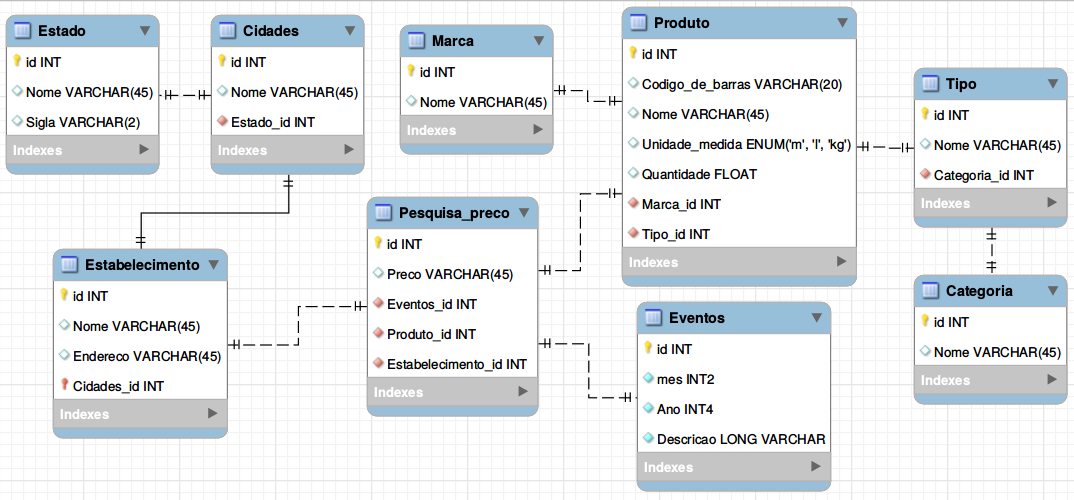
\includegraphics[width=16.0cm, height= 9.0cm]{cestadiagrama.png}    % The printed column width is 8.4 cm.
			\caption{Diagrama de Banco de Dados.} 
			\label{fig:faces}
		\end{center}
	\end{figure}
As informações foram colocadas de forma a relacionar o máximo possível, mesmo o sistema atendendo atualmente somente a cidade de paraíso foi colocado cidade e estado para que se o sistema for expandir para outras localidades o banco já está configurado.

Os produtos foram separados das marcas para facilitar na mineração de dados futuramente, para que se tenha uma noção de preferência sobre os gostos dos consumidores, pois um dos objetivos futuros quando o sistema já tiver uma boa quantidade de dados é fazer mineração de dados.

Após a finalização da decisão do banco de dados foi para o desenvolvimento do sistema Web, onde a tecnologia escolhida foi o framework Django que é escrito em Python. Esse framework foi escolhido por padronização do IFTO, onde é preferencialmente que se desenvolva aplicações utilizando esse framework.

O Django possui uma estrutura bem simples de utilização, criando o arquivo de Model e descrevendo toda a modelagem do banco de dados na sua tela administrador onde é possível fazer toda a gerência dos dados, sem precisar programar toda a estrutura do CRUD.

	\begin{figure}[H]
	\begin{center}
		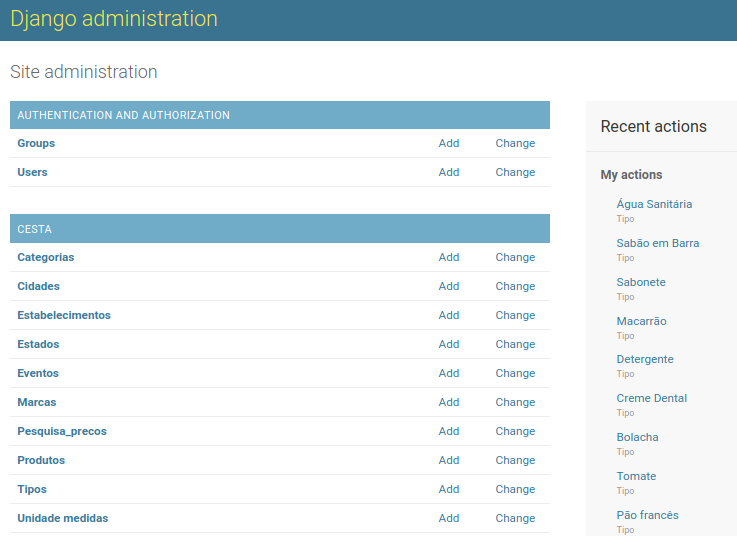
\includegraphics[width=16.0cm, height= 9.0cm]{cestaadmin.png}    % The printed column width is 8.4 cm.
		\caption{Tela administrador do Django.} 
		\label{fig:faces}
	\end{center}
\end{figure}
Com isso foi aproveitado a parte de gerência de dados e usuários, não sendo necessário programar essa parte, no entanto para quem vai pesquisar os preços utilizando essa estrutura não ficaria fácil, pois seria necessário ter que fazer vários relacionamentos de dados manualmente.

Para quem faz a pesquisa de preço foi programado um módulo que facilite, de forma de inicialmente ele pudesse escolher a data, o estabelecimento, o tipo do produto, com isso ele só irá precisar escolher o produto e colocar o preço.

	\begin{figure}[H]
	\begin{center}
		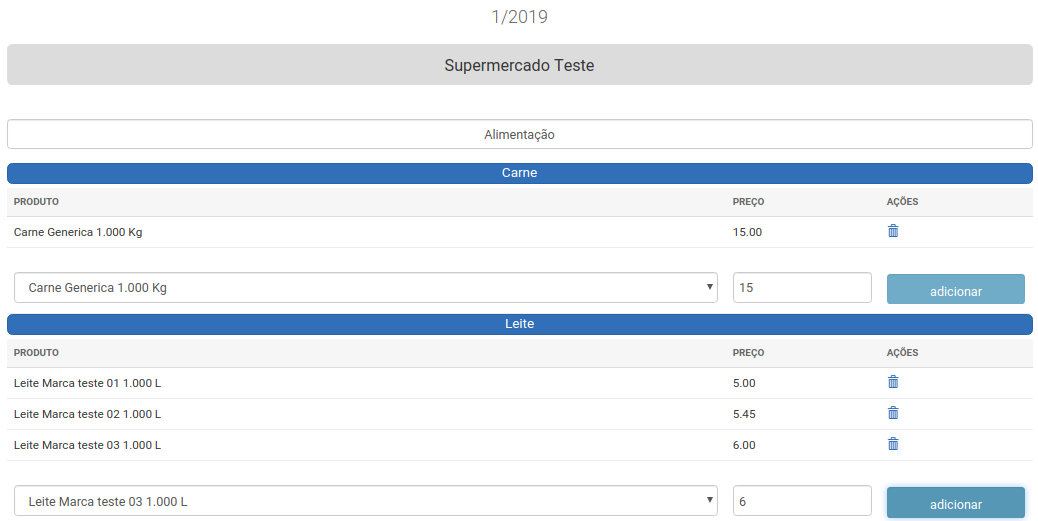
\includegraphics[width=16.0cm, height= 9.0cm]{cestacadastro.png}    % The printed column width is 8.4 cm.
		\caption{Tela de Registro de Preços Pequisados} 
		\label{fig:faces}
	\end{center}
\end{figure}

Para o Layout do visitante foi planejado um template amigável e responsivo de forma que pudesse se adaptar a qualquer resolução de tela.
	\begin{figure}[!h]
	\begin{center}
		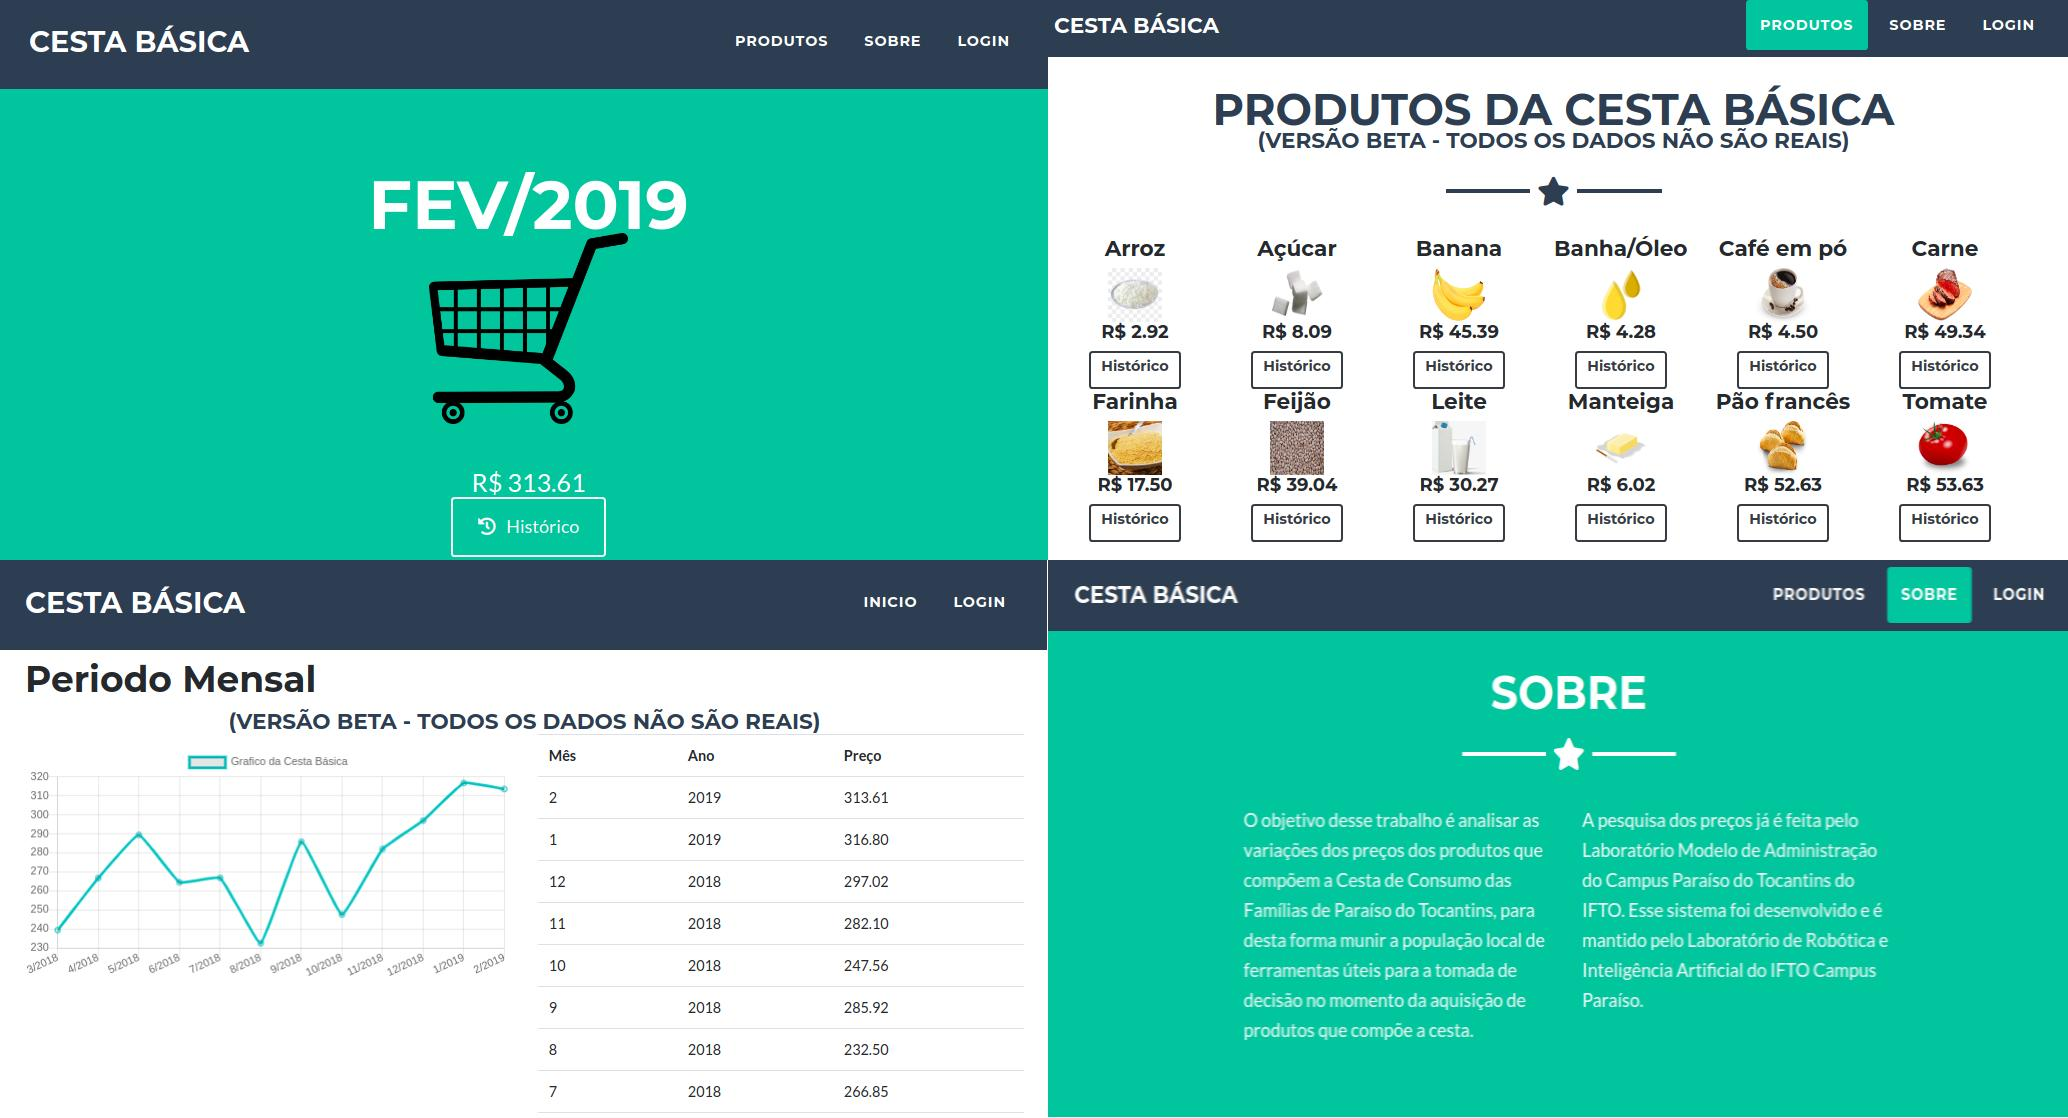
\includegraphics[width=16.0cm, height= 9.0cm]{cestauser.jpeg}    % The printed column width is 8.4 cm.
		\caption{Tela de para visualização dos dados para os usuários} 
		\label{fig:faces}
	\end{center}
\end{figure}

Após a conclusão final da versão Web do sistema será iniciado a criação do aplicativo, a proposta da criação é para que se possa ter esses dados mesmo sem internet e através da câmera do dispositivo ser capaz de ler o código de barras do produto localizá-lo suas informações.
Para que se possa desenvolver o aplicativo será necessário criar uma API dentro do framework Django, no entanto ele já oferece suporte para criação de forma simplificada.

	\begin{figure}[!h]
	\begin{center}
		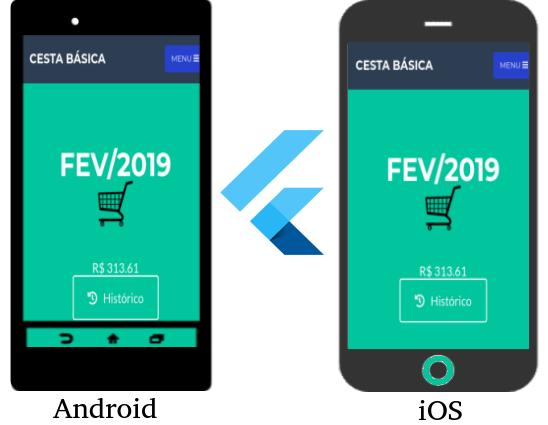
\includegraphics[width=12.0cm, height= 9.0cm]{cestadispositovos.jpeg}    % The printed column width is 8.4 cm.
		\caption{Demostração do sistema Web rodando em disposítivos móveis} 
		\label{fig:faces}
	\end{center}
\end{figure}

A tecnologia escolhida para o desenvolvimento é o Flutter, pois é uma framework que permite desenvolvimento multiplataforma, assim irá permitir que tanto os usuários do Android e iOS possam utilizar.

\chapter{Cronograma}
O desenvolvimento deste projeto está dimensionado de acordo com as seguintes atividades:
\begin{table}[h]
	\begin{tabular}{|c|c|c|c|c|c|}
		\hline
		Atividade                             & Agosto & Setembro & Outubro & Novembro & Dezembro \\
		\hline
		Conclusão da Aplicação Web            & X      & X        &         &          &          \\
		\hline
		Liberação da Aplicação Web &        & X        &         &          &          \\
		\hline
		Desenvolvimento do Aplicativo          &        & X        & X       & X        &          \\
		\hline
		Liberação do Aplicativo &        &          &         & X        &          \\
		\hline
		Integração, teste e correções         &        & X        &         & X        & X        \\
		\hline
		Revisão bibliográfica                 & X      & X        & X       & X        & X        \\
		\hline
		Redação da Monografia                 &        &          & X       & X        & X       \\
		\hline
	\end{tabular}
\caption{Cronograma}
\end{table}

% Finaliza o bookmarking do PDF
\phantompart

\begin{itemize}[label={$\bullet$}]
	\item Conclusão da Aplicação Web:
	
	Fazer os ajustes e alterações necessárias para conclusão de versão de produção da aplicação.
	
	\item Liberação da Aplicação Web:
	
	Hospedagem e divulgação da plataforma para que a população possa acessar.
	
	\item Desenvolvimento do Aplicativo:
	
	Utilizando o Flutter será feito o desenvolvimento do aplicativo
	
	\item Liberação do Aplicativo:
	
	Com a finalização do aplicativo será disponibilizado para a população baixar atrás da loja oficial da plataforma, a versão para Android será liberada primeiro, a versão para iOS será liberada depois.
	
	\item Integração, teste e correções
	Será feitos os testes necessários para saber se as aplicações não estão apresentando erros, também será corrigido caso os usuários notifiquem bugs.
	
	
\end{itemize}

% Introduz a parte pós-textual
\postextual

% Insere as referências bibliográficas
\bibliography{bibliografia}

\end{document}
